%-------------------------------------------------------------------------------
%-------------------------------------------------------------------------------
\begin{frame}
	\textbf{The Mirrlees Review} \\ \vspace{15pt}
	\begin{quote}
		The Mirrlees Review brought together a high-profile group of
		international experts and early career researchers to identify the
		characteristics of a good tax system for any open developed economy in
		the 21st century, assess the extent to which the UK tax system conforms
		to these ideals, and recommend how it might realistically be reformed in
		that direction.
	\end{quote}
\end{frame}
%-------------------------------------------------------------------------------
%-------------------------------------------------------------------------------
\begin{frame}
	\begin{figure}
		\caption{The Mirrlees Review}
		\centering
		\subfloat[]{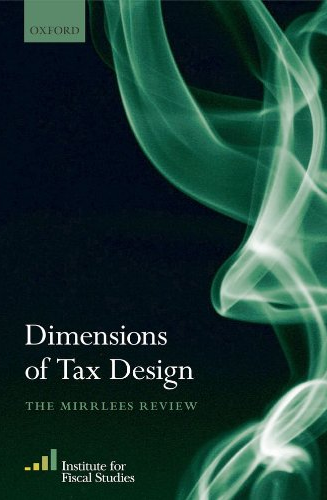
\includegraphics[width=0.40\linewidth]{fig-mirrlees-review-1}} \hspace{25pt}
		\subfloat[]{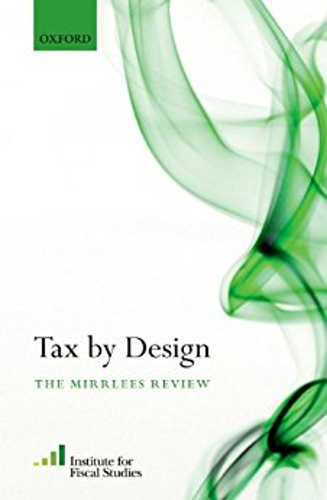
\includegraphics[width=0.40\linewidth]{fig-mirrlees-review-2}}
	\end{figure}
\end{frame}

\begin{frame}
	\begin{itemize}\setlength\itemsep{1em}
		\item \textbf{Taxation of Earnings}\medskip
		\begin{itemize}\setlength\itemsep{1em}
			\item A single integrated benefit should be introduced to replace all or most of the current multiplicity of benefits, rationalising the way in which total support varies with income and other characteristics.
		\end{itemize}
		\item \textbf{Indirect Taxes}\medskip
		\begin{itemize}\setlength\itemsep{1em}
			\item VAT should be extended to nearly all spending. This would reduce complexity and avoid costly distortions to consumption choices.
		\end{itemize}
	\end{itemize}
\end{frame}
%-------------------------------------------------------------------------------
%-------------------------------------------------------------------------------
\begin{frame}
	\begin{itemize}\setlength\itemsep{1em}
		\item \textbf{Environmental Taxes}\medskip
		\begin{itemize}\setlength\itemsep{1em}
			\item We should work towards a comprehensive system of congestion charging on the roads, replacing most of fuel duty.
		\end{itemize}
		\item \textbf{Taxes on Saving}\medskip
		\begin{itemize}\setlength\itemsep{1em}
			\item The risk-free return to saving should not be taxed, so that saving is not discouraged.
		\end{itemize}
		\item \textbf{Business Taxes}\medskip
		\begin{itemize}\setlength\itemsep{1em}
			\item The tax treatment of employment, self-employment and corporate source income should be aligned.
		\end{itemize}
	\end{itemize}
\end{frame}
